\section{Introduction}
\begin{frame}{Introduction}{}
\begin{block}{Standard \emph{shapes} of information security:}
	\begin{itemize}
		\item Confidentiality
		\item Integrity
		\item Availability
	\end{itemize}
\end{block}
	There is a new security that we want to obtain: \textbf{Anonymity}
\begin{quote}
	Anonymity [...] means that the personal identity,
	or personally identifiable information of that person is not known.
\end{quote}
\end{frame}

\begin{frame}{Introduction}{anonymity methods}
There are a lot of anonymity driven software online, like \textit{i2p},
\textit{freenet} or \textit{Tor}, we will talk about the last one because
is the most used and expanded in the real world
(2 million of client per day!).
\end{frame}

\begin{frame}{Onion Routing}{}
The onion routing model is a way to gain anonymity on the net:
\begin{itemize}
	\item Provides anonymity
	\item Protects from sniffing
\end{itemize}
Introduced by David Goldshlag, Paul Syverson and Michael Reed in the 1999.
\\
It recalls an onion because every step \textbf{peel} a layer.
\\
Let us see an implementation.
\end{frame}

\begin{frame}{Tor}{The onion router}
\begin{block}{Overview}
Tor is a group of volunteers that operates to defend anonymity online.\\
The system is based on an interconnection of machines, called \textbf{routers}.\\
It operates over the network level 4.
\end{block}
It operates as follow:
\end{frame}

\begin{frame}{Tor}{Tor workings}
\begin{center}
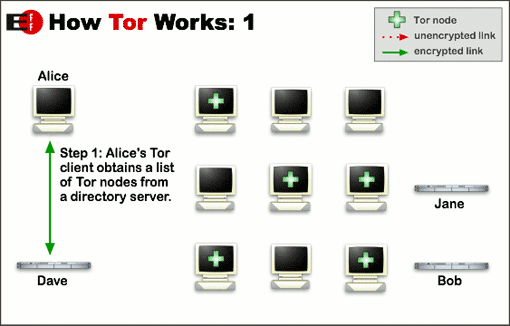
\includegraphics[scale=0.54]{img/tor1.png}
\end{center}
\end{frame}

\begin{frame}{Tor}{Tor workings}
\begin{center}
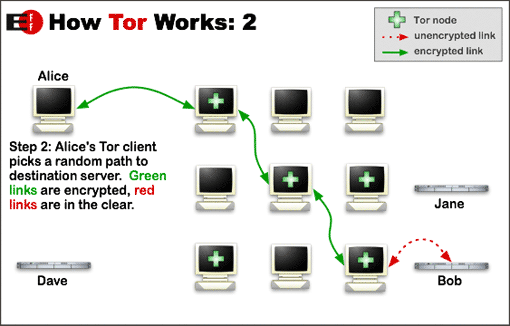
\includegraphics[scale=0.54]{img/tor2.png}
\end{center}
\end{frame}

\begin{frame}{Tor}{Tor workings}
\begin{center}
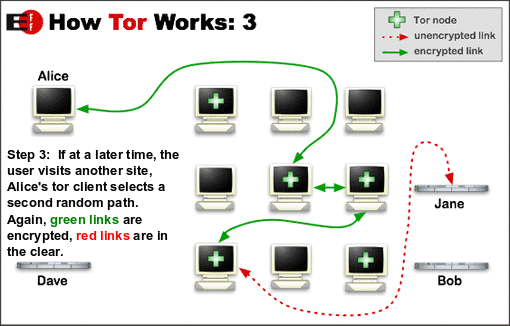
\includegraphics[scale=0.72]{img/tor3.png}
\end{center}
\end{frame}

\begin{frame}{Tor}{Tor encryption}
\begin{center}
	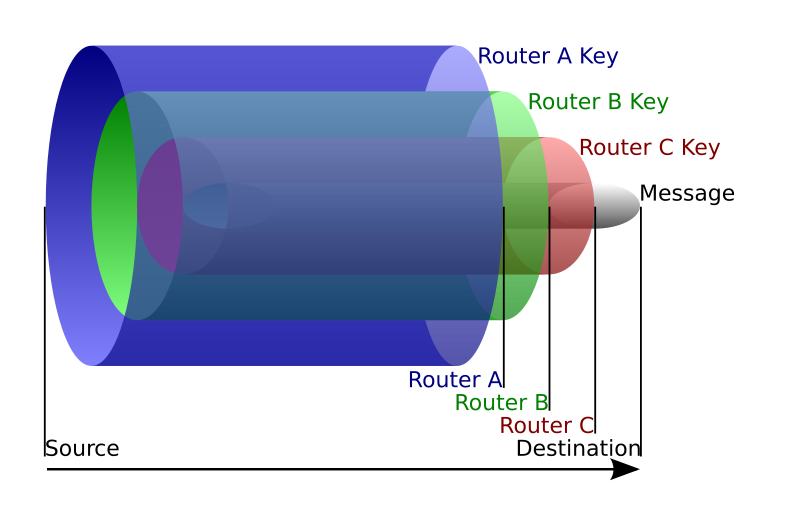
\includegraphics[scale=0.35]{img/onion.png}
\end{center}
\end{frame}

\begin{frame}{Tor}{Tor encryption}
\begin{center}
	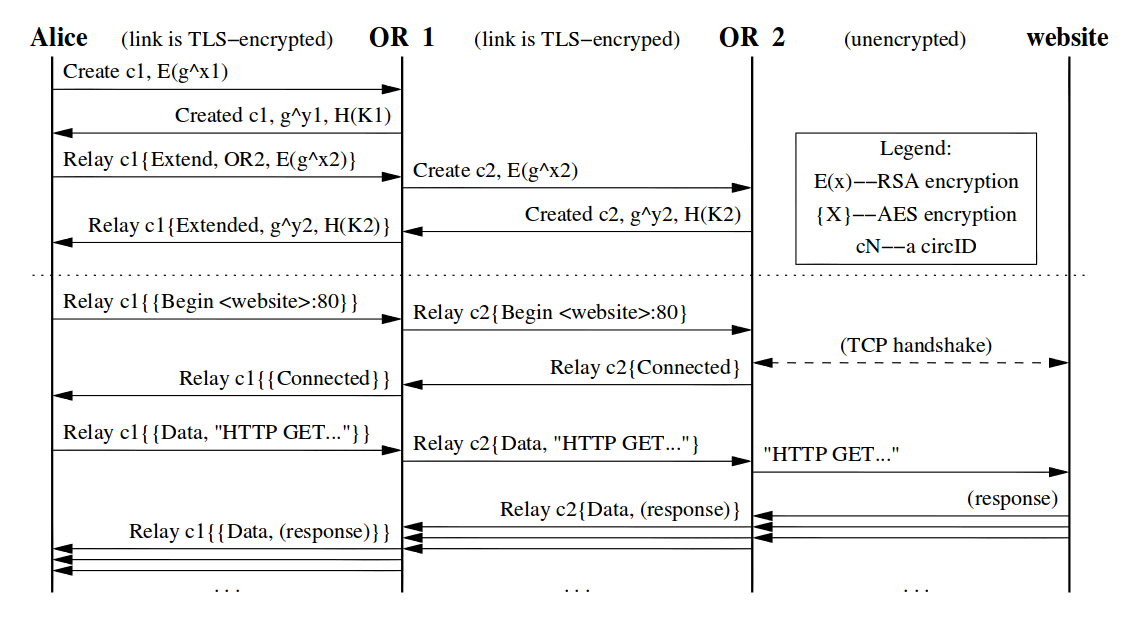
\includegraphics[scale=0.28]{img/or-communication.png}
\end{center}
\end{frame}
\subsection{Attacks}
\begin{frame}{Attacks}{}
	A lot of attacks and vulnerabilities has been discovered for the system.
	\begin{itemize}
		\item Bad apple attack.
		\item Side channel attacks (tor bundle).
		\item Cypher attacks (Tor changed the cryptosystem a lot of time).
		\item \emph{Time analysis based attacks}
		\item Sniper attack.
		\item Sybil attack.
	\end{itemize}
\end{frame}

\begin{frame}{Time analysis based attacks}{}
	\begin{quote}
		\emph{``Tor does not provide protection against end-to-end timing attacks[...]''}
	\end{quote}
	We can place a tracker after the client node and another before the server node
	and check for the connection time to profile users and nodes (and later associate IP to users.)
\end{frame}

\section{Simulation}
\begin{frame}{Simulation}{}
	\begin{itemize}
		\item From this idea we started our simulation work.
		\item But \textbf{OmNet++} doesn't have a reliable simulation
		      model of Tor\footnote{And Tor is fully implemented in
		      User-Space (over level 4)} and so \textbf{NS2/3}.
		\item We needed a simulation model for Tor.
	\end{itemize}
\end{frame}

\subsection{Shadow}
\begin{frame}{Shadow}{Introduction}
	\begin{itemize}
		\item We used the \textbf{Shadow} simulator
		\item Developed by \textbf{Rob Jansen} (U.S. Naval Research Lab).
	\end{itemize}
	\begin{block}{Users}
		
\includegraphics[width=\textwidth]{img/shadow-users.png}
	\end{block}
\end{frame}

\begin{frame}{Shadow}{Simulator internals}
	\begin{minipage}{\textwidth}
	The main feature of \textbf{shadow} is the capability of running real
	applications (like tor).
	\end{minipage}
	\begin{minipage}{0.45\textwidth}
	\small
	Shadow combines virtualization with simulation, it virtualize network
	stacks and act as an micro system hypervisor (partial virtualization).
	\normalsize
	\end{minipage}
	\begin{minipage}{0.4\textwidth}
	\begin{center}
		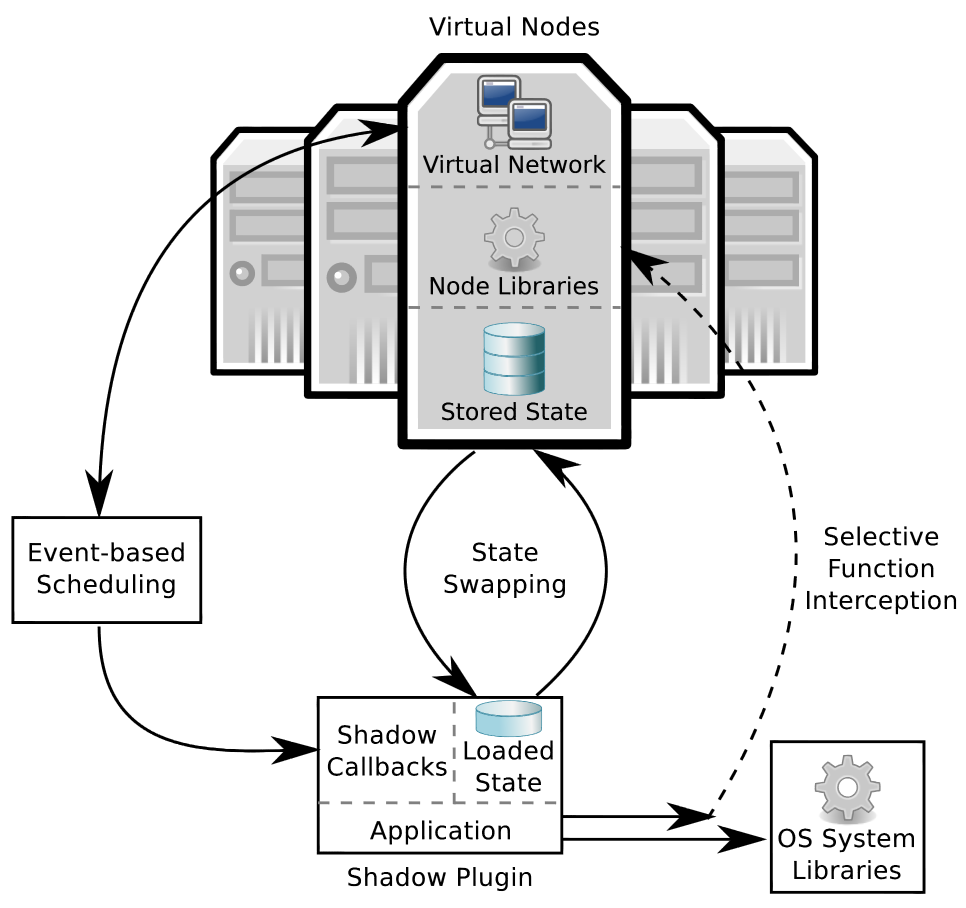
\includegraphics[scale=0.17]{img/shadow.png}
	\end{center}
	\end{minipage}
\end{frame}

\subsection{Plug-ins}

\begin{frame}{Plug-ins}{Shadow plugins}
\end{frame}

